% !Mode:: "TeX:UTF-8"
% !TEX program  = xelatex
\section{Performance assessment}
\subsection{Visualization}
To evaluate the performance of ZIVA, we tested the visualization result of ZIVA and six other popular methods including PCA [], tSNE [], UMAP [], ZIFA [], VASC [] and ivis [] on 6 datasets with different number of cells and different sequencing protocols (Table \ref{datasets}). The visualization result is shown in Figure \ref{vis}.
\begin{figure}[htb!]
    \centering
    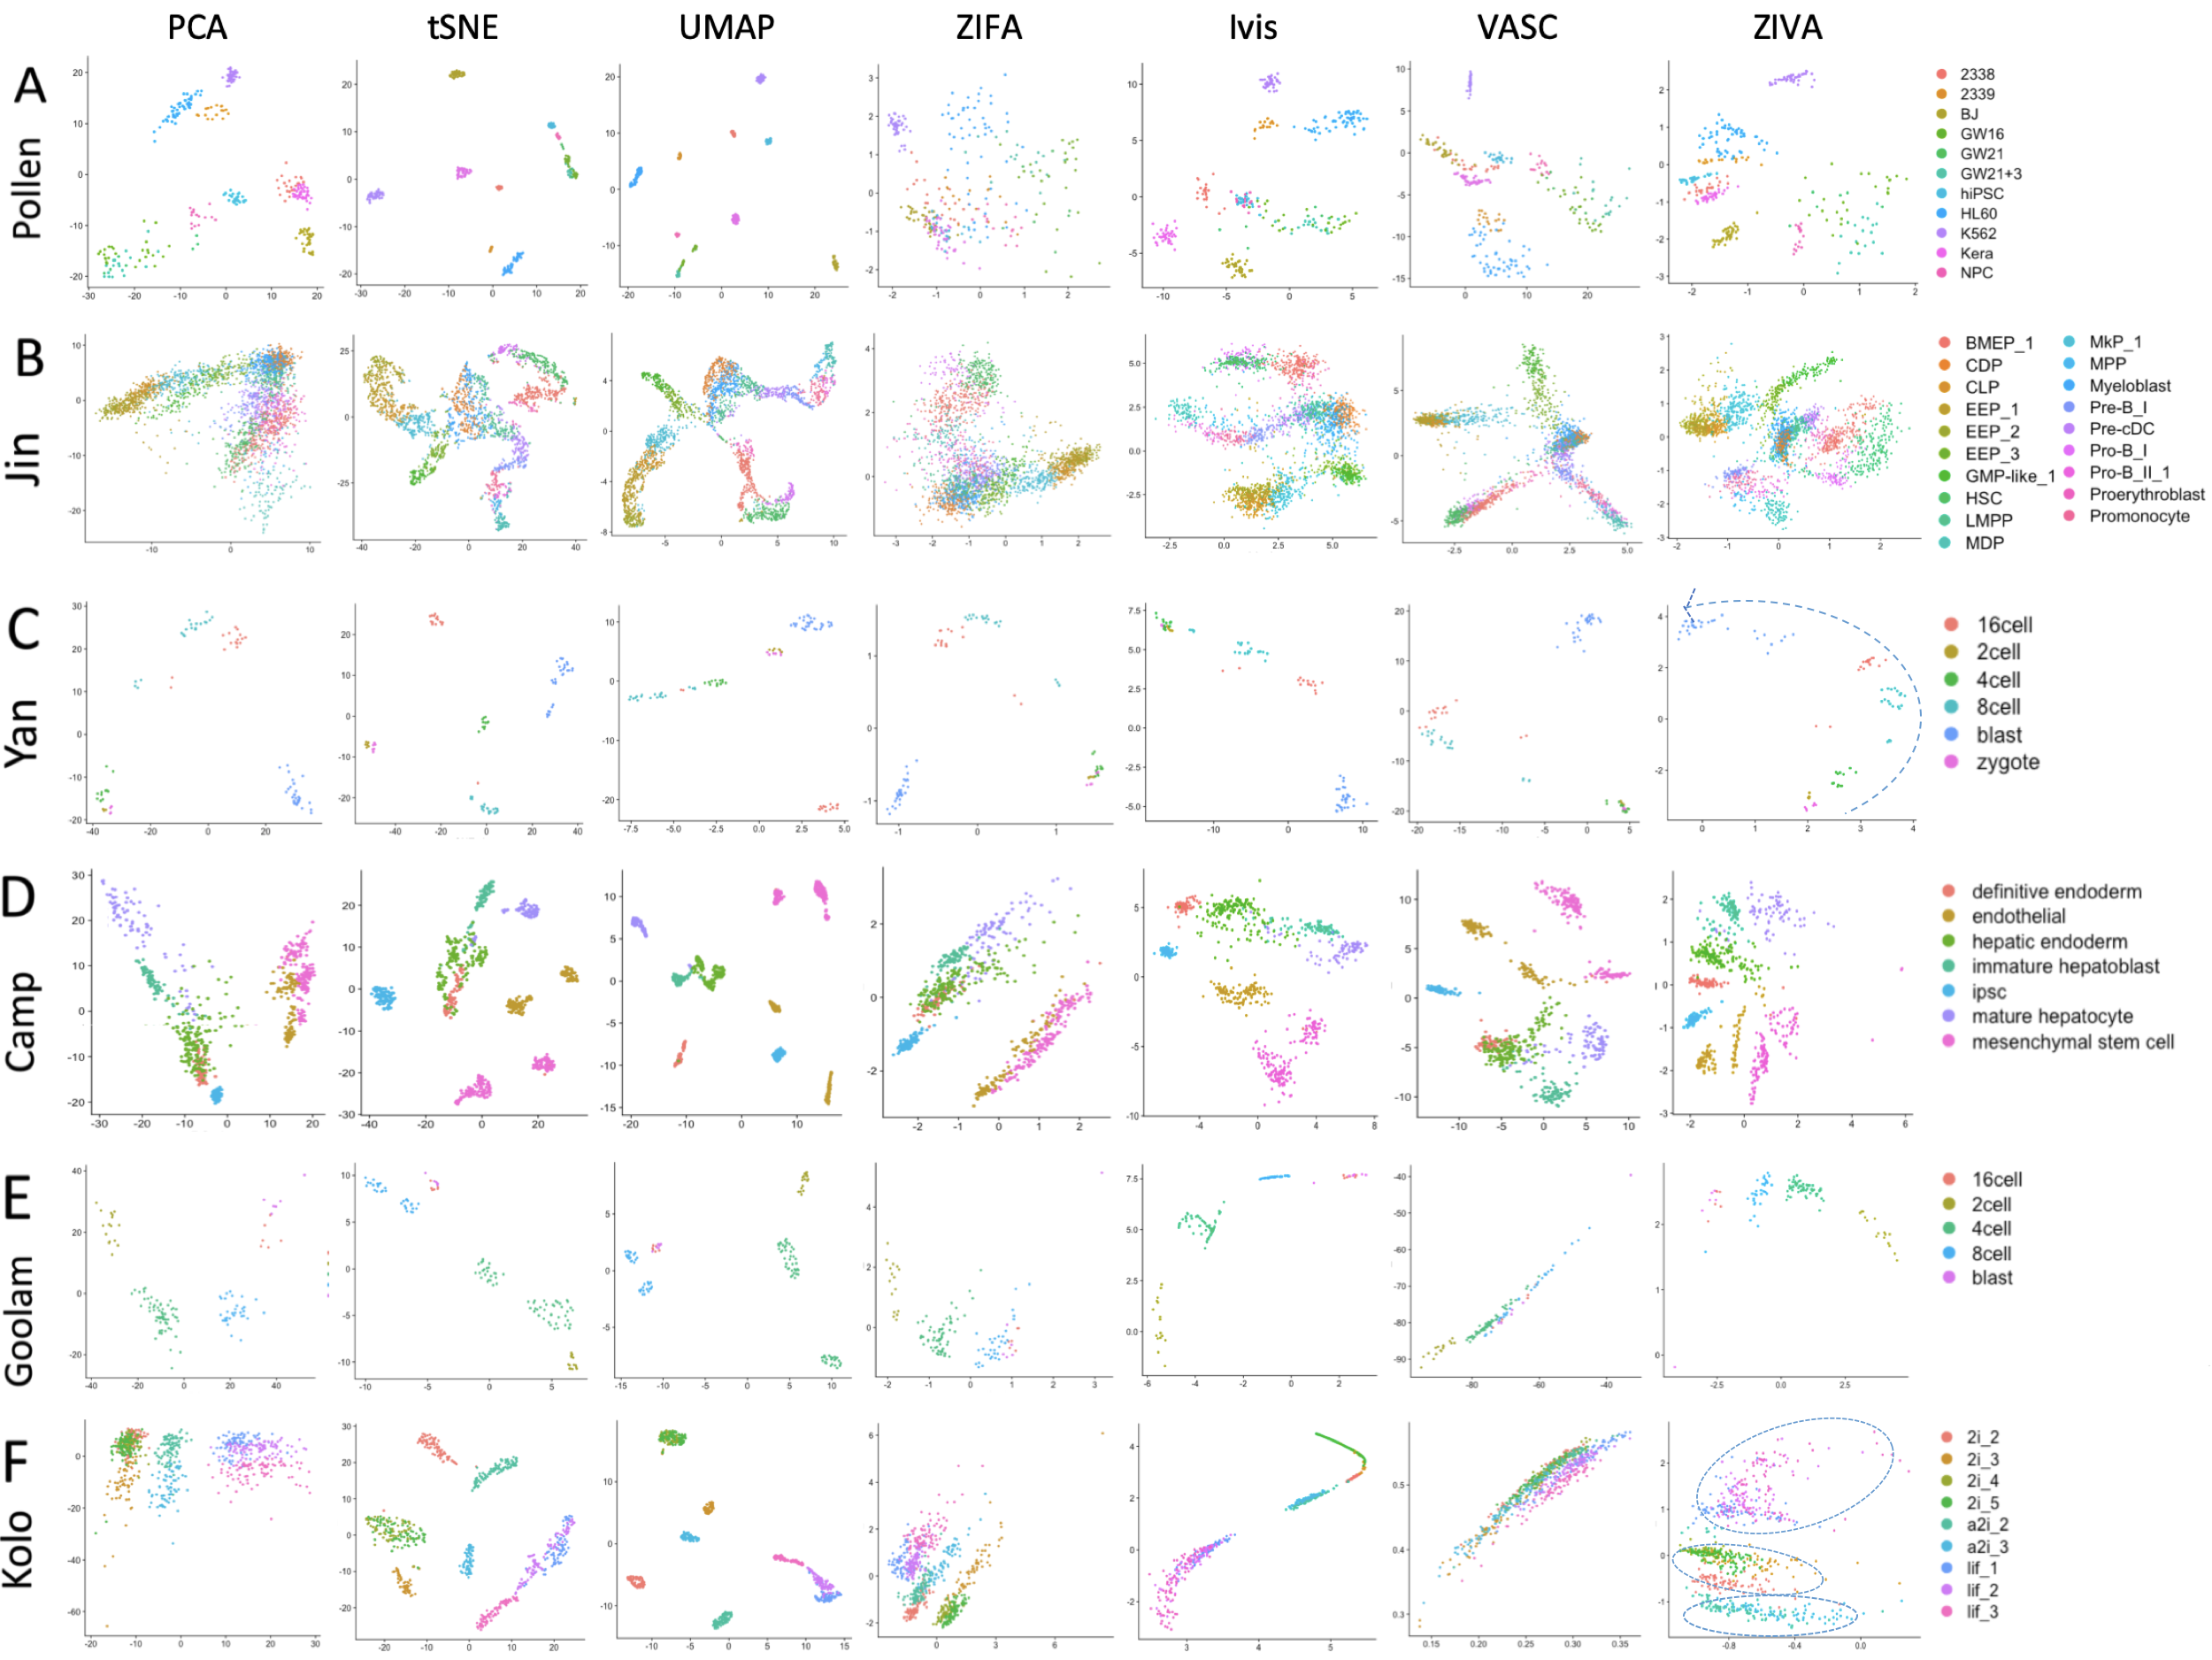
\includegraphics[width=1\textwidth]{figures/myfigures/visualizations.png}
    \caption{Visualization of scRNA-seq datasets}
    \label{vis}
\end{figure}
The results show that ZIVA has great performance all of six datasets. The clusters in the datasets can be well identified and cell lineages are also well recovered. For example, the Pollen dataset (Figure2.A) contains eleven different types of cells including blood, dermal, neural and pluripotent cells. ZIVA and most other methods except ZIFA can clearly separate them to different clusters. \\
The Yan dataset (Figure2.C) contains several types of embryonic cells from zygote to blast. VASC not only separate different cell types perfectly, but also greatly reconstructed the developmental stages of the cells. We can tell the developmental lineage (zygote, 2cell, 4cell, 8cell, 16cell, blast) from the visualization by ZIVA. PCA, Ivis, VASC and ZIFA also generated the lineage structure, but not as clear as in ZIVA. However, tSNE and UMAP that focus on local structure didn’t successfully recover the developmental relationships. It shows that ZIVA has superior performance on modelling embryo development progression than ZIFA, tSNE and UMAP. \\
The Kolodziejczyk dataset contains the embryonic cells grown from three different conditions: serum, 2i and alternate 2i (a2i). Under each condition, there are different batches of cells. It can be seen that ZIVA, Ivis and ZIFA well separated different culture conditions and several batches. PCA can also separate the conditions but batches are slightly mixed. VASC generated a mussy result. tSNE and UMAP formed beautiful clusters but failed to distinguish three conditions.
\subsection{Clustering performance}
Next, to quantitatively measure the performance of different methods, we evaluate the result of visualization by applying clustering to the dimensionality reduced 2D data. We used K-means to cluster cells and set k to the number of known cell types. Then, we compared the clustering results to the ground truth clusters that are annotated in the original papers. We used the normalized mutual information (NMI) and the adjusted rand index (ARI) to evaluate the performance of different methods. 

\vspace{0.5cm}
\noindent\emph{NMI} \\
Suppose T is the true cell types, P is the predicted cell types, H(X) means the entropy of X, n is the number of all samples and MI(A,B) means the mutual information between A and B. Then, NMI is computed as following:
\begin{equation}
    NMI(P, T)=\frac{MI(P, T)}{\sqrt{H(P) H(T)}}
\end{equation}

\vspace{0.5cm}
\noindent\emph{ARI} \\
Suppose n is the number of total cells, ai is the number of cells that are clustered to the i-th cluster pf P, bj is the number of cells that belong to the j-th cell types in T. nij is the number of cells that overlap the i-th cluster in P and j-th cell types in T. Then, ARI can be computed as following:
\begin{equation}
    ARI = \frac{\sum_{i j}\left(\begin{array}{c}n_{i j} \\ 2\end{array}\right)-\frac{\left[\sum_{i}\left(\begin{array}{c}a_{i} \\ 2\end{array}\right) \sum_{j}\left(\begin{array}{c}b_{j} \\ 2\end{array}\right)\right]}{\left(\begin{array}{l}n \\ 2\end{array}\right)}}{\frac{1}{2}\left[\sum_{i}\left(\begin{array}{c}a_{i} \\ 2\end{array}\right)+\sum_{j}\left(\begin{array}{c}b_{j} \\ 2\end{array}\right)\right]-\frac{\left[\sum_{i}\left(\begin{array}{c}a_{i} \\ 2\end{array}\right) \sum_{j}\left(\begin{array}{c}b_{j} \\ 2\end{array}\right)\right]}{\left(\begin{array}{l}n \\ 2\end{array}\right)}}
\end{equation}
The results are shown in Table \ref{nmiall} and Table \ref{ariall}. In some cases, ZIVA outperforms other methods such as the dataset5. However, sometimes ZIVA doesn't perform well on clustering tasks.
\begin{table}[htb!]
\centering
\caption{NMI of each dataset on different methods}
\label{nmiall}
\resizebox{10cm}{!}{
\begin{tabular}{llllllll}
\hline
  & PCA  & tSNE & UMAP & ZIFA & VASC & Ivis & ZIVA \\ \hline
1 & 0.88 & 0.92 & 0.92 & 0.60 & 0.79 & 0.86 & 0.84 \\
2 & 0.57 & 0.67 & 0.71 & 0.59 & 0.65 & 0.65 & 0.67 \\
3 & 0.79 & 0.87 & 0.91 & 0.79 & 0.75 & 0.81 & 0.79 \\
4 & 0.70 & 0.78 & 0.81 & 0.60 & 0.72 & 0.81 & 0.66 \\
5 & 0.86 & 0.73 & 0.73 & 0.76 & 0.48 & 0.94 & 0.94 \\
6 & 0.70 & 0.84 & 0.87 & 0.66 & 0.25 & 0.65 & 0.60 \\ \hline
\end{tabular}}
\end{table}

\begin{table}[htb!]
\centering
\caption{ARI of each dataset on different methods}
\label{ariall}
\resizebox{13cm}{!}{
\begin{tabular}{llllllll}
\hline
  & PCA  & tSNE & UMAP & ZIFA & VASC & Ivis & ZIVA \\ \hline
1 & 0.79 & 0.84 & 0.84 & 0.44 & 0.65 & 0.80 & 0.73 \\
2 & 0.34 & 0.41 & 0.48 & 0.36 & 0.39 & 0.39 & 0.43 \\
3 & 0.63 & 0.78 & 0.90 & 0.63 & 0.60 & 0.74 & 0.64 \\
4 & 0.56 & 0.61 & 0.64 & 0.42 & 0.54 & 0.70 & 0.47 \\
5 & 0.71 & 0.54 & 0.54 & 0.75 & 0.45 & 0.97 & 0.98 \\
6 & 0.48 & 0.74 & 0.77 & 0.48 & 0.11 & 0.48 & 0.43 \\ \hline
\end{tabular}}
\end{table}

\subsection{Trajectory inference performance assessment}
Next, we tested the performance of ZIVA for trajectory cells. We used a dataset for pancreatic a and b cell development. They performed the single cell RNA sequencing at several developmental stages of E17.5, P0, P3, P9, P15, P18 and P60 of $a-$ and $b-$ cells that were sorted from mouse strains by fluorescence-activated cell sorting. We performed the PCA, tSNE, UMAP, Ivis and ZIVA to that datasets. The result shows that ZIVA can successfully recover the developmental lineage from both a- and b- pancreatic cells (Figure \ref{traj}). Other methods can also separate two cell types but contains more mixed points.  
\begin{figure}[htb!]
    \centering
    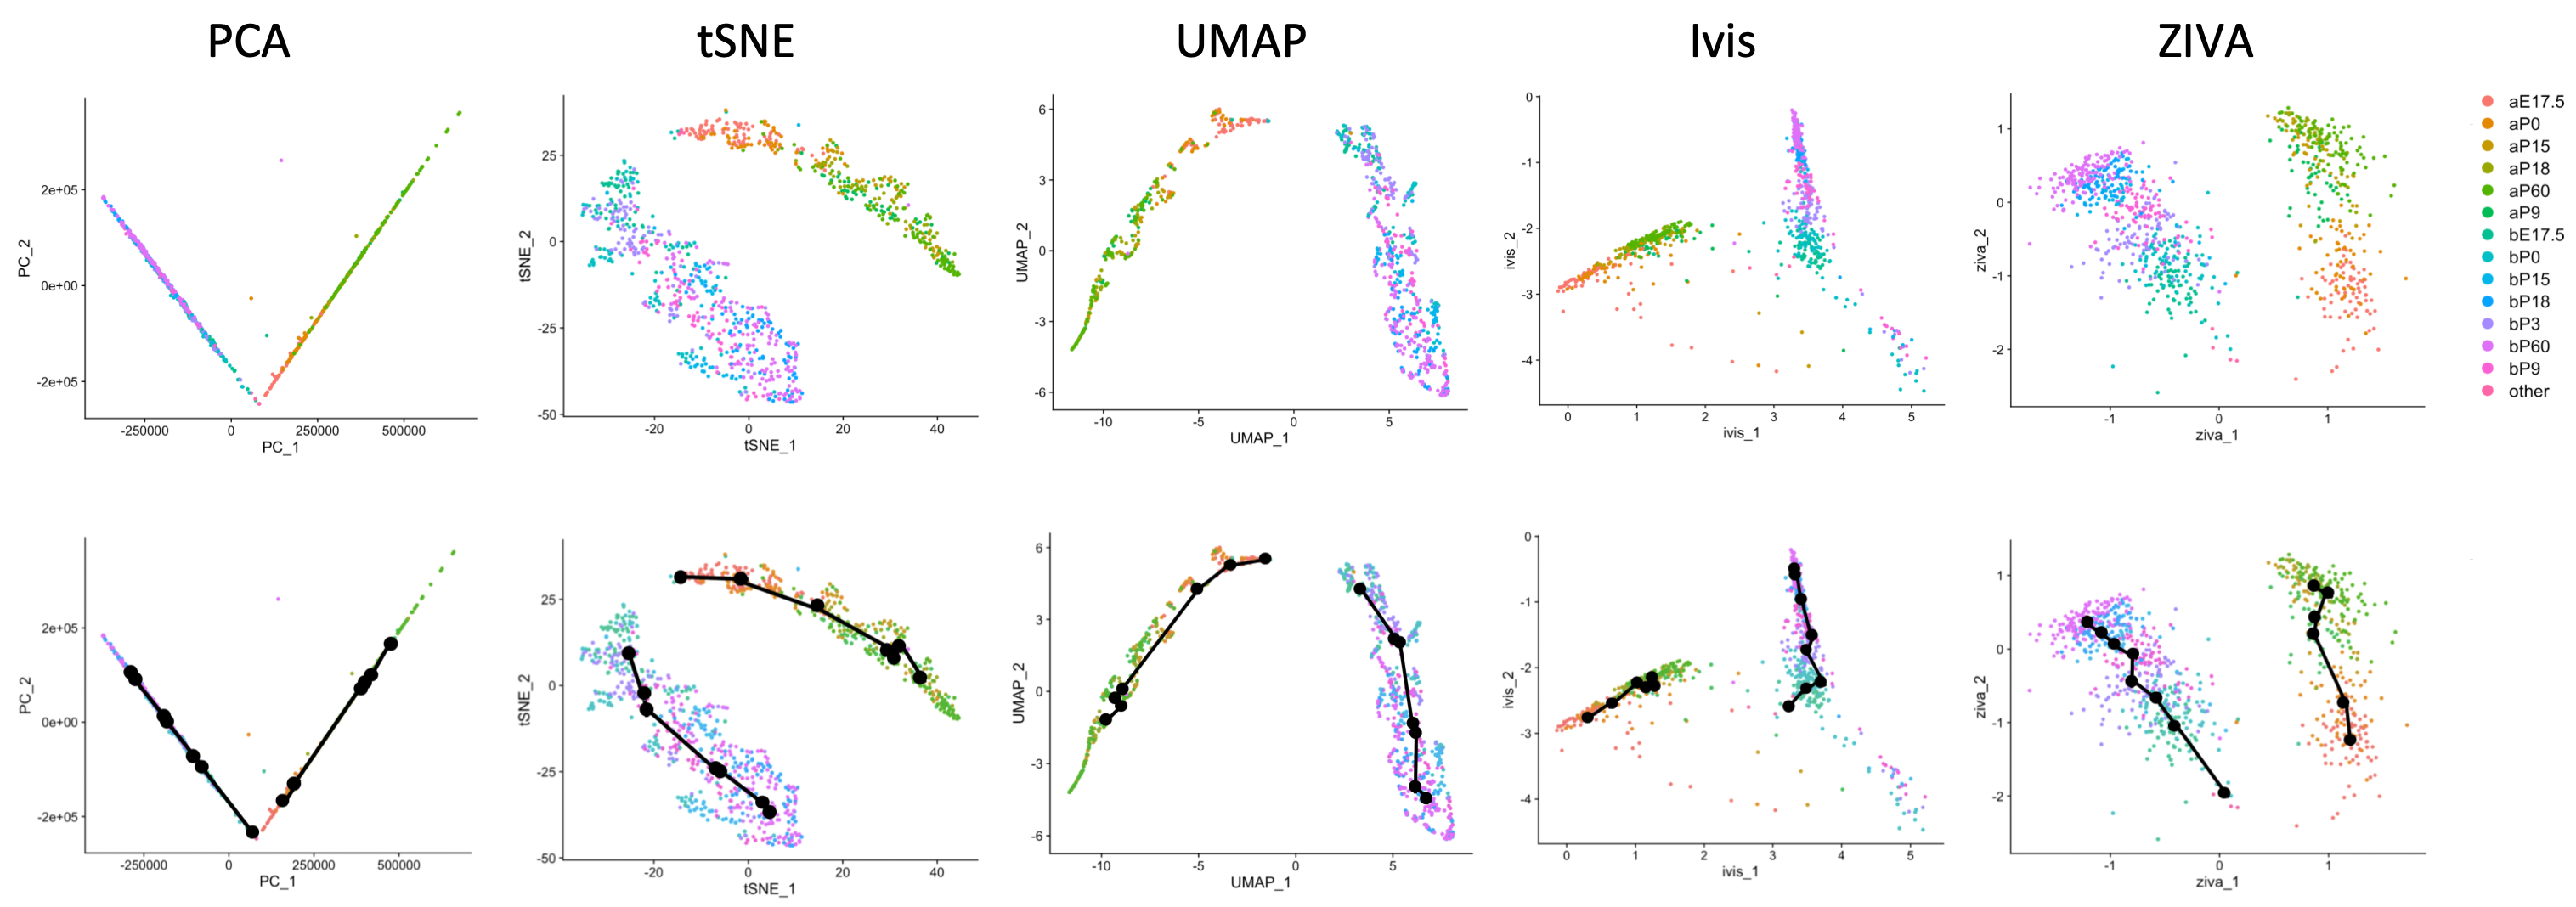
\includegraphics[width=1\textwidth]{figures/myfigures/traj.png}
    \caption{P}
    \label{}
\end{figure}

